\subsection{Riepilogo complessivo}
\subsubsection{Ore totali}
Di seguito vengono riportate le tabelle delle ore totali utilizzate per il progetto con i relativi costi; sono considerate sia quelle d'investimento che quelle rendicontate.

\begin{minipage}[b]{0.65\linewidth}
\begin{small}
{
\setlength\arrayrulewidth{.8pt}
\begin{longtable}{ c | c c c c c c | c} 
 \rowcolor{coloreRosso}
 \color{white}{\textbf{Nominativo}} &
 \color{white}{\textbf{RE}} &
 \color{white}{\textbf{AM}} &
 \color{white}{\textbf{AN}} &
 \color{white}{\textbf{PT}} &
 \color{white}{\textbf{PR}} &
 \color{white}{\textbf{VE}} &
 \color{white}{\textbf{Tot.}} \\
 	
 \BM{} & 14 & 19 & 19 & 20 & 28 & 32 & 132 \\ 
 \SG{} & 11 & 15 & 18 & 22 & 34 & 32 & 132 \\ 
 \SH{} & 6 & 13 & 22 & 22 & 36 & 33 & 132 \\ 
 \PA{} & 12 & 22 & 7 & 23 & 30 & 38 & 132 \\ 
 \SP{} & 8 & 17 & 22 & 21 & 27 & 37 & 132 \\ 
 \RA{} & 14 & 16 & 15 & 23 & 27 & 37 & 132 \\ 
 \ZM{} & 12 & 20 & 18 & 19 & 29 & 34 & 132 \\
 
 	\rowcolor{coloreRosso}
 	\color{white}{\textbf{Ore totali/ruolo}} &
 	\color{white}{\textbf{77}} &
 	\color{white}{\textbf{122}} &
 	\color{white}{\textbf{121}} &
 	\color{white}{\textbf{150}} &
 	\color{white}{\textbf{211}} &
 	\color{white}{\textbf{243}} &
 	\color{white}{\textbf{924}} \\
 	\rowcolor{white}
 	\captionsetup{width=.9\textwidth}
 	\caption{Distribuzione delle ore totali d'investimento e rendicontate}
\end{longtable}
}
\end{small}
\end{minipage}
\begin{minipage}[b]{.3\linewidth}
\begin{small}
{
\setlength\arrayrulewidth{.7pt}
\begin{longtable}{ c | c | c} 
 	\rowcolor{coloreRosso}
 	\color{white}{\textbf{Ruolo}} &
 	\color{white}{\textbf{Ore}} &
 	\color{white}{\textbf{Costo €}} \\
 	
 	Responsabile & 77 & 2310\\
 	Amministratore & 122 & 2440\\
 	Analista & 121 & 3025\\
 	Progettista & 150 & 3300\\
 	Programmatore & 211 & 3165\\
 	Verificatore & 243 & 3645\\
 	
 	\rowcolor{coloreRosso}
 	\color{white}{\textbf{Totale}} &
 	\color{white}{\textbf{924}} &
 	\color{white}{\textbf{17885 €}}\\
 	\rowcolor{white}
 	\caption{Prospetto dei costi delle ore totali di investimento e rendicontate}
\end{longtable}
}
\end{small}
\end{minipage}

I seguenti grafici riassumo i dati ottenuti.

\begin{figure}[!htb]
   \begin{minipage}{0.6\textwidth}
     \centering
     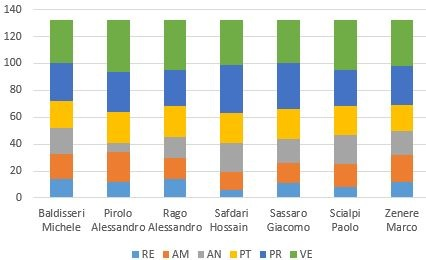
\includegraphics{Images/PO-OreTotali}
     \caption{Ripartizione oraria totale per ciascun membro}
   \end{minipage}\hspace{0.1\textwidth}
   \begin{minipage}{0.3\textwidth}
     \centering
     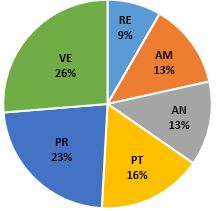
\includegraphics[width=.9\textwidth]{Images/PE-OreTotali}
     \captionsetup{width=.9\textwidth}
     \caption{Ripartizione ore totali}
   \end{minipage}
\end{figure}

\subsubsection{Ore rendicontate}
Di seguito vengono riportate le tabelle delle ore totali \textbf{rendicontate}, ovvero quelle a carico del committente.

\begin{minipage}[b]{0.65\linewidth}
\begin{small}
{
\setlength\arrayrulewidth{.8pt}
\begin{longtable}{ c | c c c c c c | c} 
 \rowcolor{coloreRosso}
 \color{white}{\textbf{Nominativo}} &
 \color{white}{\textbf{RE}} &
 \color{white}{\textbf{AM}} &
 \color{white}{\textbf{AN}} &
 \color{white}{\textbf{PT}} &
 \color{white}{\textbf{PR}} &
 \color{white}{\textbf{VE}} &
 \color{white}{\textbf{Tot.}} \\
 	
 \BM{} & - & 19 & 7 & 20 & 28 & 28 & 102 \\ 
 \SG{} & - & 15 & 5 & 22 & 34 & 26 & 102 \\ 
 \SH{} & 6 & 6 & 5 & 22 & 36 & 27 & 102 \\ 
 \PA{} & 12 & 8 & 5 & 23 & 30 & 24 & 102 \\ 
 \SP{} & 8 & 17 & - & 21 & 27 & 29 & 102 \\ 
 \RA{} & 14 & 4 & 11 & 23 & 27 & 23 & 102 \\ 
 \ZM{} & 12 & 8 & 10 & 19 & 29 & 24 & 102 \\
 
 	\rowcolor{coloreRosso}
 	\color{white}{\textbf{Ore totali/ruolo}} &
 	\color{white}{\textbf{52}} &
 	\color{white}{\textbf{77}} &
 	\color{white}{\textbf{43}} &
 	\color{white}{\textbf{150}} &
 	\color{white}{\textbf{211}} &
 	\color{white}{\textbf{181}} &
 	\color{white}{\textbf{714}} \\
 	\rowcolor{white}
 	\captionsetup{width=.9\textwidth}
 	\caption{Distribuzione delle ore totali rendicontate}
\end{longtable}
}
\end{small}
\end{minipage}
\begin{minipage}[b]{.3\linewidth}
\begin{small}
{
\setlength\arrayrulewidth{.7pt}
\begin{longtable}{ c | c | c} 
 	\rowcolor{coloreRosso}
 	\color{white}{\textbf{Ruolo}} &
 	\color{white}{\textbf{Ore}} &
 	\color{white}{\textbf{Costo €}} \\
 	
 	Responsabile & 52 & 1560\\
 	Amministratore & 77 & 1540\\
 	Analista & 43 & 1075\\
 	Progettista & 150 & 3300\\
 	Programmatore & 211 & 3165\\
 	Verificatore & 181 & 2715\\
 	
 	\rowcolor{coloreRosso}
 	\color{white}{\textbf{Totale}} &
 	\color{white}{\textbf{714}} &
 	\color{white}{\textbf{13355 €}}\\
 	\rowcolor{white}
 	\caption{Prospetto dei costi delle ore totali rendicontate}
\end{longtable}
}
\end{small}
\end{minipage}

I seguenti grafici riassumo i dati ottenuti.

\begin{figure}[!htb]
   \begin{minipage}{0.6\textwidth}
     \centering
     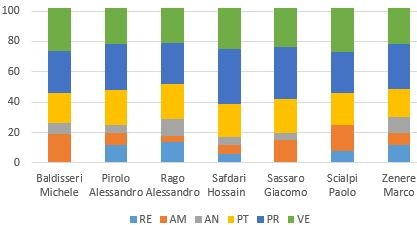
\includegraphics{Images/PO-OreRendicontate}
     \caption{Ripartizione delle ore rendicontate per ciascun membro}
   \end{minipage}\hspace{0.1\textwidth}
   \begin{minipage}{0.3\textwidth}
     \centering
     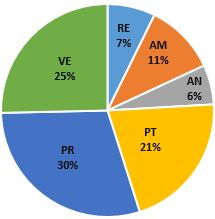
\includegraphics[width=.9\textwidth]{Images/PE-OreRendicontate}
     \captionsetup{width=.9\textwidth}
     \caption{Ripartizione ore rendicontate}
   \end{minipage}
\end{figure}

